\subsubsection{Разработка модели системы}

\paragraph{Модуль рубрикатора новостей и сохранённых запросов.} \hfill

Диаграмма прецедентов для данного модуля представлена на рис.~\ref{figure:activityRubricator}.
\begin{figure}[h!]
\centering
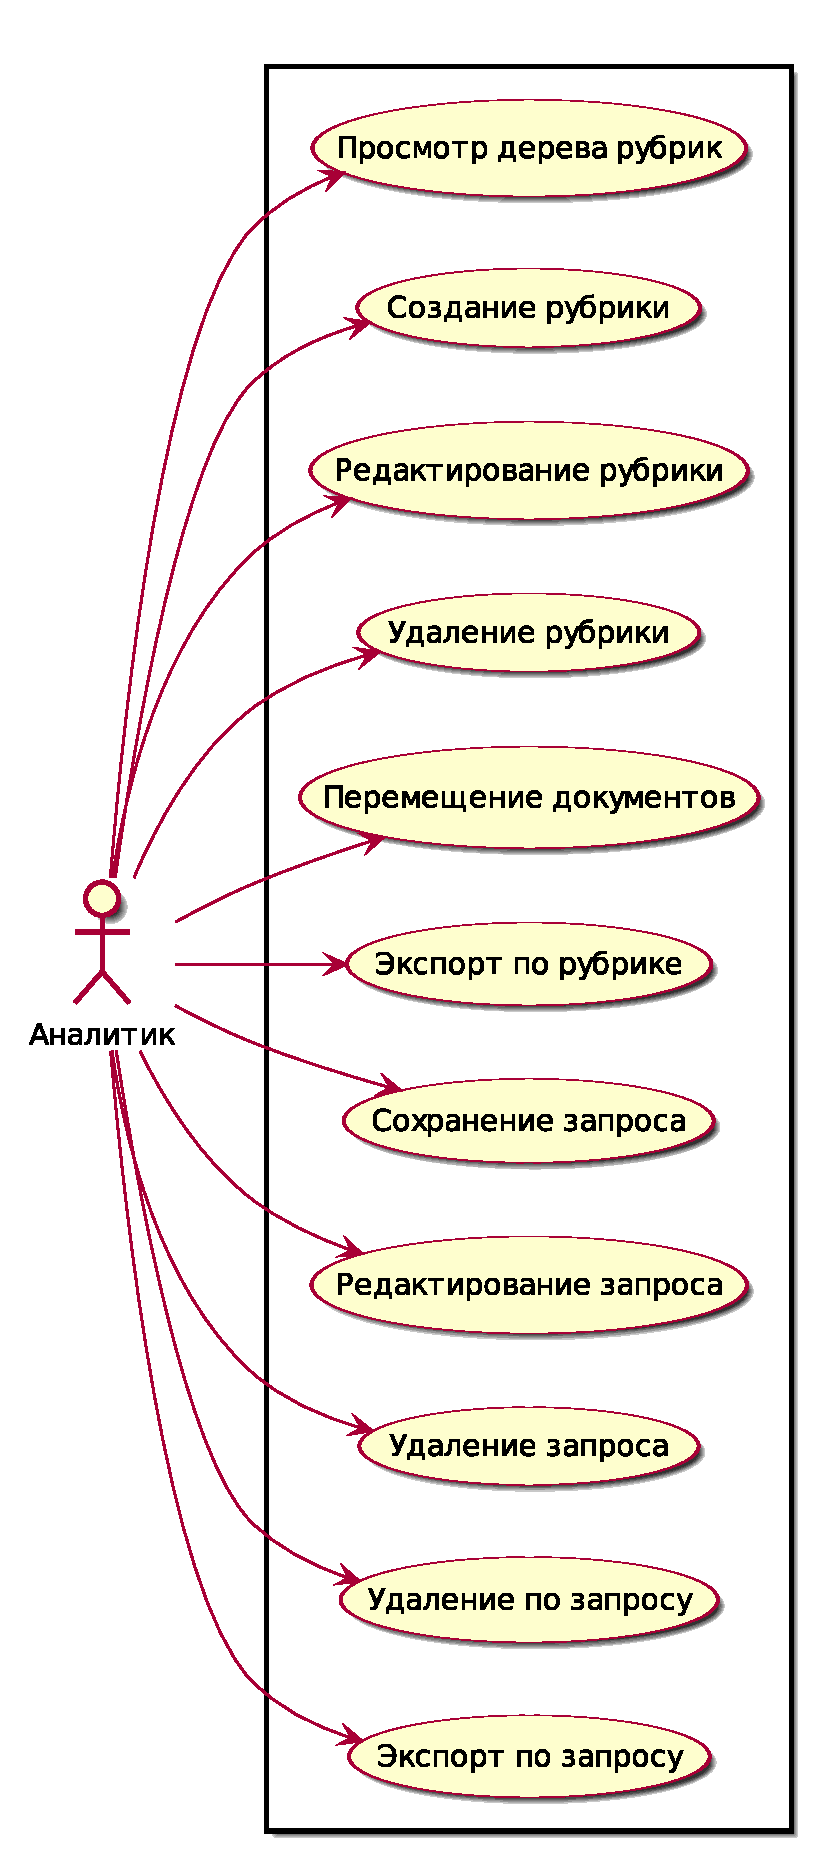
\includegraphics[height=0.8\textheight]{design/rubricator_usecase}
\caption{Диаграмма прецедентов для рубрикатора}
\label{figure:activityRubricator}
\end{figure}

\clearpage
\paragraph{Модуль поиска новостей и формализованных запросов.} \hfill


\clearpage
\paragraph{Модуль просмотра новости.} \hfill


\clearpage
\paragraph{Модуль управления индексом.} \hfill


\clearpage
\paragraph{Модуль интеграционного интерфейса.} \hfill


\clearpage
\paragraph{Модуль настроек системы.} \hfill


\clearpage
\paragraph{Модуль добавления документов.} \hfill


\clearpage
\paragraph{Модуль прогнозирования.} \hfill


\clearpage
\paragraph{Модуль индексирования.} \hfill